\documentclass[11pt,a4paper]{article}

\usepackage[utf8]{inputenc}
\usepackage[T1]{fontenc}
\usepackage{mathpazo}
\usepackage[scaled=0.92]{helvet}
\usepackage[margin=1in]{geometry}
\usepackage{graphicx}
\usepackage{amsmath,amssymb,amsfonts}
\usepackage{booktabs}
\usepackage{tabularx}
\usepackage{setspace}
\usepackage{titlesec}
\usepackage{fancyhdr}
\usepackage{float}
\usepackage{caption}
\usepackage{listings}
\usepackage{microtype}
\usepackage{tikz}
\usepackage{xcolor}
\usepackage[hidelinks]{hyperref}

\usetikzlibrary{shapes.geometric, arrows.meta, positioning, calc, matrix, fit, backgrounds}

\setstretch{1.15}
\setlength{\parindent}{0pt}
\setlength{\parskip}{0.8em}
\sloppy

\titleformat{\section}{\normalfont\large\bfseries\sffamily}{\thesection}{1em}{}
\titleformat{\subsection}{\normalfont\normalsize\bfseries\sffamily}{\thesubsection}{1em}{}
\titleformat{\subsubsection}{\normalfont\normalsize\itshape\sffamily}{\thesubsubsection}{1em}{}

\pagestyle{fancy}
\fancyhf{}
\fancyhead[L]{\small\sffamily libvctrl API Developer Reference}
\fancyhead[R]{\small\sffamily\thepage}
\renewcommand{\headrulewidth}{0.4pt}

\captionsetup{font=small,labelfont=bf,labelsep=period}

\renewenvironment{abstract}
{\small
	\begin{center}\textbf{\sffamily Abstrak}\end{center}
	\begin{quote}}
	{\end{quote}}

\lstdefinestyle{code}{
	basicstyle=\ttfamily\footnotesize,
	frame=single,
	rulecolor=\color{black},
	breaklines=true,
	showstringspaces=false,
	columns=fullflexible,
	keepspaces=true,
	framesep=6pt,
	aboveskip=1em,
	belowskip=1em,
	xleftmargin=0pt
}

\lstdefinestyle{out}{
	basicstyle=\ttfamily\footnotesize,
	frame=tb,
	rulecolor=\color{black},
	breaklines=true,
	showstringspaces=false,
	columns=fullflexible,
	keepspaces=true,
	framesep=4pt,
	aboveskip=1em,
	belowskip=1em
}

\title{\vspace{-1.5cm}\textbf{\sffamily\LARGE Referensi API \href{https://docs.rs/libvctrl/2.2.1}{libvctrl@2.2.1}\\ Untuk Pengembang Integrasi dan Backend}}
\author{
	\textbf{Muhammad Riduwan Khafidi} \\
	\small Program Studi Teknik Rekayasa Perangkat Lunak \\
	\small Politeknik Negeri Batam \\
	\small \texttt{4342611034@students.polibatam.ac.id}
}
\date{\small\today}

\begin{document}

\maketitle
\thispagestyle{empty}

\begin{abstract}
	libvctrl adalah workspace Rust untuk membangun sistem kendali versi yang dapat dikustomisasi. Dokumen ini menyajikan spesifikasi API publik workspace untuk pengembang yang akan memakai, memperluas, atau mengimplementasikan ulang kontraknya. Cakupan meliputi lapisan kontrak, implementasi referensi, primitif kriptografi, fasad, plumbing, dan backend penyimpanan. Setiap API dijelaskan melalui tanda tangan fungsi, batasan tipe, kondisi error, dan kontrak thread safety. Dokumen memuat tujuh visualisasi TikZ, dua belas tabel spesifikasi, dan blok kode yang dapat dikompilasi terhadap crate versi yang tercantum. Pengembang memperoleh referensi presisi untuk integrasi dan ekstensi tanpa menebak perilaku runtime.
\end{abstract}

\section{Pendahuluan}

\subsection{Motivasi Pengembang}

Seorang pengembang yang membangun sistem kendali versi kustom menghadapi empat keputusan yang tidak boleh salah: bagaimana objek direpresentasikan, bagaimana objek diserialisasi, bagaimana objek di-address secara kriptografis, dan bagaimana objek disimpan. libvctrl memisahkan keempat keputusan itu ke dalam empat lapisan yang dapat dipilih secara independen. Lapisan kontrak mendefinisikan representasi. Lapisan implementasi referensi mendefinisikan serialisasi dan addressing. Lapisan kriptografi menyediakan primitif. Lapisan backend mendefinisikan penyimpanan.

Pemisahan ini hanya bernilai jika pengembang dapat melihat batas setiap lapisan tanpa membaca kode sumber. Dokumen ini menyajikan batas itu secara eksplisit: tanda tangan fungsi lengkap dengan bound generik, kondisi error yang mungkin, dan invariant yang dijamin oleh konstruktor.

\subsection{Audiens dan Asumsi}

Dokumen ini ditujukan untuk pengembang Rust dengan pemahaman tentang trait, generik, lifetime, dan operator \texttt{?}. Dokumen mengasumsikan pembaca pernah memakai \texttt{cargo}, memahami perbedaan antara \texttt{std::io::Read} dan \texttt{std::io::BufRead}, serta mengenal pola builder. Dokumen tidak mengajarkan dasar Rust. Dokumen tidak mengajarkan dasar sistem kendali versi.

\subsection{Peta Pembahasan}

Bagian kedua memetakan arsitektur workspace dan kontrak thread safety. Bagian ketiga membahas tipe dan trait kontrak. Bagian keempat membahas format biner byte-level. Bagian kelima membahas implementasi referensi. Bagian keenam membahas primitif kriptografi. Bagian ketujuh membahas fasad dan plumbing. Bagian kedelapan membahas template implementasi backend kustom. Bagian kesembilan menyajikan studi kasus end-to-end. Bagian kesepuluh merangkum kesalahan umum, dan bagian kesebelas memberikan lembar rujukan cepat.

\section{Arsitektur Workspace}

\subsection{Graf Ketergantungan}

Workspace libvctrl disusun satu arah. \texttt{libvctrl\_handler} tidak bergantung pada crate lain di workspace. \texttt{libvctrl\_core} bergantung pada \texttt{libvctrl\_handler} dan \texttt{libvctrl\_sha512}. Fasad \texttt{libvctrl} mengekspor ulang ketiganya. \texttt{libvctrl\_plumbing} dibangun di atas \texttt{libvctrl\_core} dan \texttt{libvctrl}. Backend seperti \texttt{libvctrl\_monumentum} mengimplementasikan trait dari \texttt{libvctrl\_handler} dan bergantung pada engine penyimpanan eksternal.

Gambar~\ref{fig:arsitektur} menunjukkan arah ketergantungan. Panah berarti ``bergantung pada''.

\begin{figure}[H]
	\centering
	\resizebox{\textwidth}{!}{%
	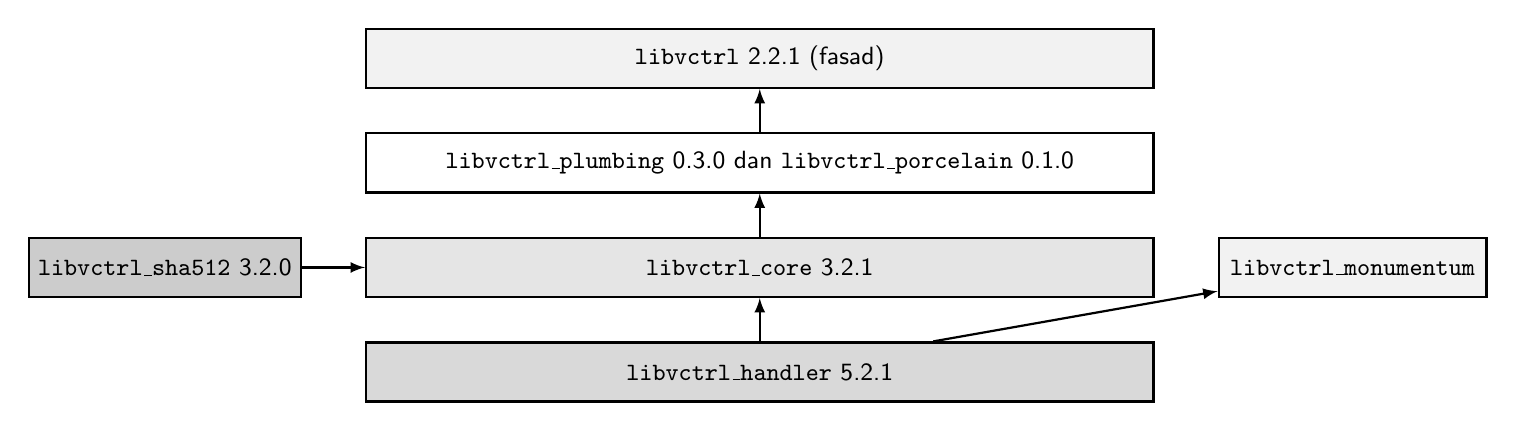
\begin{tikzpicture}[
			node distance=0.55cm,
			box/.style={rectangle, draw=black, thick, minimum width=10cm, minimum height=0.75cm, align=center, font=\sffamily\small},
			side/.style={rectangle, draw=black, thick, minimum width=3.4cm, minimum height=0.75cm, align=center, font=\sffamily\small},
			line/.style={draw, thick, -latex}
		]
		\node[box, fill=black!5] (facade) {\texttt{libvctrl} 2.2.1 (fasad)};
		\node[box, fill=white, below=of facade] (plumbing) {\texttt{libvctrl\_plumbing} 0.3.0 dan \texttt{libvctrl\_porcelain} 0.1.0};
		\node[box, fill=black!10, below=of plumbing] (core) {\texttt{libvctrl\_core} 3.2.1};
		\node[box, fill=black!15, below=of core] (handler) {\texttt{libvctrl\_handler} 5.2.1};
		\node[side, fill=black!20, left=0.8cm of core] (sha) {\texttt{libvctrl\_sha512} 3.2.0};
		\node[side, fill=black!5, right=0.8cm of core] (mon) {\texttt{libvctrl\_monumentum}};

		\draw[line] (handler) -- (core);
		\draw[line] (core) -- (plumbing);
		\draw[line] (plumbing) -- (facade);
		\draw[line] (sha) -- (core);
		\draw[line] (handler) -- (mon);
	\end{tikzpicture}%
	}
	\caption{Arah ketergantungan antarcrate dalam workspace libvctrl.}
	\label{fig:arsitektur}
\end{figure}

\subsection{Tabel Crate}

Tabel~\ref{tab:crate} merangkum versi, peran, MSRV, dan lisensi setiap crate.

\begin{table}[H]
	\centering
	\caption{Metadata crate pada workspace libvctrl.}
	\label{tab:crate}
	\footnotesize
	\begin{tabularx}{\textwidth}{l l X l l}
		\toprule
		Crate & Versi & Peran & MSRV & Lisensi \\
		\midrule
		\texttt{libvctrl} & 2.2.1 & Fasad re-export & 1.96.0 & MIT \\
		\texttt{libvctrl\_handler} & 5.2.1 & Kontrak, tipe, validasi & 1.96.0 & MIT \\
		\texttt{libvctrl\_core} & 3.2.1 & Codec, builder, store & 1.96.0 & MIT \\
		\texttt{libvctrl\_sha512} & 3.2.0 & SHA-512, HMAC, HKDF & 1.96.0 & ISC \\
		\texttt{libvctrl\_plumbing} & 0.3.0 & Operasi perintah & 1.96.0 & MIT \\
		\texttt{libvctrl\_porcelain} & 0.1.0 & API tingkat tinggi & 1.96.0 & MIT \\
		\texttt{libvctrl\_monumentum} & 0.1.0 & Backend Monumentum & 1.96.0 & MIT \\
		\bottomrule
	\end{tabularx}
\end{table}

\subsection{Kontrak Thread Safety}

Seluruh trait operasi pada \texttt{libvctrl\_handler} mendeklarasikan supertrait \texttt{Send + Sync}. Konsekuensinya: implementasi backend dapat dipakai lintas thread tanpa pembungkus tambahan. Operasi baca menerima \texttt{\&self}; operasi tulis menerima \texttt{\&mut self}. Tipe data immutable seperti \texttt{Hash}, \texttt{Blob}, dan \texttt{Tree} secara otomatis \texttt{Send + Sync} karena hanya memuat \texttt{Vec}, \texttt{String}, dan array.

Gambar~\ref{fig:thread} menunjukkan aliran bound dari trait ke tipe turunan.

\begin{figure}[H]
	\centering
	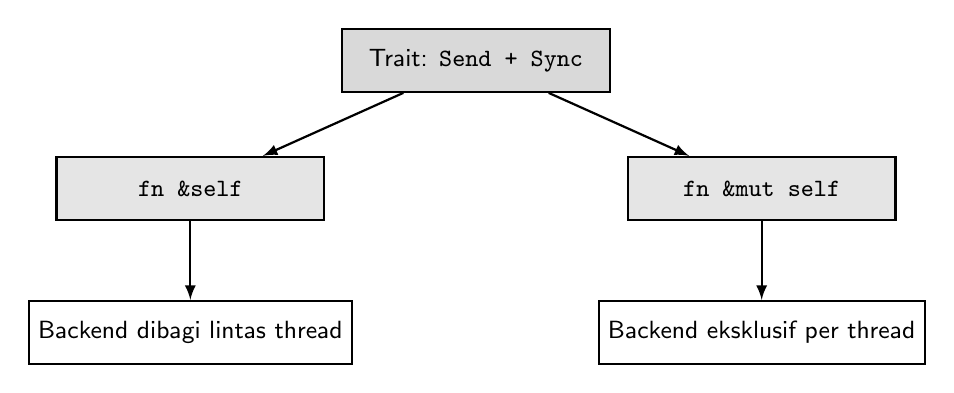
\begin{tikzpicture}[
			node distance=0.7cm and 1.2cm,
			box/.style={rectangle, draw=black, thick, minimum width=3.4cm, minimum height=0.8cm, align=center, font=\sffamily\small},
			line/.style={draw, thick, -latex}
		]
		\node[box, fill=black!15] (trait) {Trait: \texttt{Send + Sync}};
		\node[box, fill=black!10, below left=0.8cm and 0.2cm of trait] (read) {\texttt{fn \&self}};
		\node[box, fill=black!10, below right=0.8cm and 0.2cm of trait] (write) {\texttt{fn \&mut self}};
		\node[box, fill=white, below=1.0cm of read] (shared) {Backend dibagi lintas thread};
		\node[box, fill=white, below=1.0cm of write] (exclusive) {Backend eksklusif per thread};

		\draw[line] (trait) -- (read);
		\draw[line] (trait) -- (write);
		\draw[line] (read) -- (shared);
		\draw[line] (write) -- (exclusive);
	\end{tikzpicture}
	\caption{Bound \texttt{Send + Sync} pada trait menentukan pola pemakaian backend.}
	\label{fig:thread}
\end{figure}

\section{Kontrak: libvctrl\_handler}

\subsection{Tipe Data dan Tanda Tangan Konstruktor}

Semua tipe data bersifat immutable setelah konstruksi. Konstruktor bersifat fallible: input divalidasi sebelum objek dibuat. Tabel~\ref{tab:tipe} mencantumkan tanda tangan konstruktor dan accessor kunci.

\begin{table}[H]
	\centering
	\caption{Tanda tangan konstruktor dan accessor tipe kontrak.}
	\label{tab:tipe}
	\footnotesize
	\begin{tabularx}{\textwidth}{l X X}
		\toprule
		Tipe & Konstruktor & Accessor kunci \\
		\midrule
		\texttt{Hash} & \texttt{from\_bytes(\&[u8]) -> Result<Self, \_>} & \texttt{as\_bytes() -> \&[u8; 64]} \\
		\texttt{Blob} & \texttt{new(Vec<u8>) -> Result<Self, \_>} & \texttt{data() -> \&[u8]}, \texttt{size() -> usize} \\
		\texttt{TreeEntry} & \texttt{new(String, EntryKind, Hash)} & \texttt{name()}, \texttt{kind()}, \texttt{hash()} \\
		\texttt{Tree} & \texttt{new(Vec<TreeEntry>)} & \texttt{entries() -> \&[TreeEntry]}, \texttt{get(\&str)} \\
		\texttt{CommitMeta} & \texttt{new(i64, i16, Option<String>)} & \texttt{timestamp()}, \texttt{timezone\_offset()} \\
		\texttt{Commit} & \texttt{new(Hash, Vec<Hash>, UserID, UserID, String)} & \texttt{tree()}, \texttt{parents()}, \texttt{author()} \\
		\texttt{Tag} & \texttt{new(String, Hash, Option<UserID>, String)} & \texttt{name()}, \texttt{target()}, \texttt{tagger()} \\
		\texttt{UserID} & \texttt{new(String, String) -> Result<Self, \_>} & \texttt{name() -> \&str}, \texttt{email() -> \&str} \\
		\texttt{ReflogEntry} & \texttt{new(Option<Hash>, Option<Hash>, String, i64, i16)} & \texttt{old\_id()}, \texttt{new\_id()}, \texttt{reason()} \\
		\bottomrule
	\end{tabularx}
\end{table}

Konstruktor \texttt{Commit::with\_meta} dan \texttt{Tag::with\_meta} menerima \texttt{CommitMeta} eksplisit. Keduanya dipakai ketika encoding atau timestamp perlu dikendalikan. Konstruktor \texttt{Commit::new} dan \texttt{Tag::new} memakai \texttt{CommitMeta::default()}.

\subsection{Trait Operasi}

Tabel~\ref{tab:trait} mencantumkan tanda tangan trait operasi yang harus diimplementasikan backend atau dipakai oleh alat.

\begin{table}[H]
	\centering
	\caption{Tanda tangan trait operasi.}
	\label{tab:trait}
	\footnotesize
	\begin{tabularx}{\textwidth}{l X}
		\toprule
		Trait & Tanda tangan metode utama \\
		\midrule
		\texttt{Encoder} & \texttt{fn encode\_blob<W: Write+Send>(\&self, \&Blob, \&mut W) -> Result<(), VctrlError>} \\
		\texttt{Decoder} & \texttt{fn decode\_blob<R: Read+Send>(\&self, R) -> Result<Blob, VctrlError>} \\
		\texttt{Hasher} & \texttt{fn hash<R: Read+Send>(\&self, R) -> Result<Hash, VctrlError>} \\
		\texttt{ObjectStore} & \texttt{put(\&mut self, \&Hash, \&[u8])}, \texttt{get(\&self, \&Hash) -> Result<Box<dyn Read+Send+'\_>, \_>} \\
		\texttt{RefStore} & \texttt{set\_ref(\&mut self, \&str, \&Hash)}, \texttt{get\_ref(\&self, \&str) -> Result<Hash, \_>} \\
		\texttt{Index} & \texttt{add(\&mut self, Self::Entry)}, \texttt{write\_tree(\&self) -> Result<Self::TreeId, \_>} \\
		\texttt{Blame} & \texttt{blame\_file(\&self, \&str) -> Result<Vec<BlameEntry>, \_>} \\
		\texttt{RevWalk} & \texttt{walk(\&self, \&Self::CommitId) -> Result<RevWalkIterator<Self::CommitId>, \_>} \\
		\texttt{TreeDiffer} & \texttt{diff\_trees(\&self, \&Self::TreeId, \&Self::TreeId) -> Result<TreeDelta, \_>} \\
		\texttt{Remote} & \texttt{fetch(\&mut self, \&[Self::RefSpec])}, \texttt{push(\&mut self, \&[Self::RefSpec])} \\
		\texttt{Transport} & \texttt{fetch\_object(\&self, \&Hash)}, \texttt{push\_object(\&mut self, \&Hash, \&[u8])} \\
		\texttt{PackReader} & \texttt{read\_object(\&self, \&Self::ObjectId) -> Result<Box<dyn Read+Send+'\_>, \_>} \\
		\texttt{PackWriter} & \texttt{write\_object(\&mut self, \&Self::ObjectId, \&[u8])} \\
		\texttt{Signer} & \texttt{sign(\&mut self, \&str, \&[u8]) -> Result<Vec<u8>, \_>} \\
		\texttt{Verifier} & \texttt{verify(\&self, \&str, \&[u8], \&[u8]) -> Result<bool, \_>} \\
		\texttt{ConfigStore} & \texttt{get\_string(\&self, \&str, \&str) -> Result<Option<String>, \_>} \\
		\texttt{ReflogStore} & \texttt{append(\&mut self, \&Self::RefName, Option<Hash>, Option<Hash>, \&str, i64, i16)} \\
		\bottomrule
	\end{tabularx}
\end{table}

Setiap trait memiliki bound \texttt{Send + Sync}. Implementasi backend wajib memenuhi bound tersebut. Untuk backend yang memakai \texttt{Arc<Mutex<E>>}, bound terpenuhi otomatis selama \texttt{E: Send}.

\subsection{Konstanta Sistem}

Tabel~\ref{tab:konstanta} mencantumkan konstanta dan nilainya. Konstanta ini dipakai oleh konstruktor untuk menolak input yang melebihi batas.

\begin{table}[H]
	\centering
	\caption{Konstanta sistem dan nilai default.}
	\label{tab:konstanta}
	\footnotesize
	\begin{tabularx}{\textwidth}{l l X}
		\toprule
		Konstanta & Nilai & Dipakai oleh \\
		\midrule
		\texttt{HASH\_LENGTH} & 64 & \texttt{Hash::from\_bytes}, \texttt{Hash::as\_bytes} \\
		\texttt{MAX\_NAME\_LENGTH} & 255 & \texttt{UserID}, \texttt{validate\_name} \\
		\texttt{MAX\_BLOB\_SIZE} & 100 $\times$ 1024$^2$ & \texttt{Blob::new} \\
		\texttt{MAX\_TREE\_ENTRIES} & 100\,000 & \texttt{Tree::new} \\
		\texttt{MAX\_MESSAGE\_LENGTH} & 1024 $\times$ 1024 & \texttt{Commit}, \texttt{Tag} \\
		\texttt{MAX\_PARENT\_COUNT} & 65\,535 & \texttt{Commit::new} \\
		\bottomrule
	\end{tabularx}
\end{table}

\subsection{Varian Error}

Semua operasi fallible mengembalikan \texttt{VctrlError}. Varian \texttt{IoError} membungkus \texttt{Arc<std::io::Error>} agar tetap \texttt{Clone}. Tabel~\ref{tab:error} mencantumkan pemicu setiap varian.

\begin{table}[H]
	\centering
	\caption{Varian \texttt{VctrlError} dan pemicunya.}
	\label{tab:error}
	\footnotesize
	\begin{tabularx}{\textwidth}{l X}
		\toprule
		Varian & Pemicu \\
		\midrule
		\texttt{CorruptedData(String)} & Byte stream tidak sesuai format, UTF-8 invalid, atau trailing bytes \\
		\texttt{DuplicateParent} & Vektor parent memuat hash yang sama lebih dari sekali \\
		\texttt{ExceededMaxSize(String)} & Panjang melebihi \texttt{MAX\_*} \\
		\texttt{InvalidBlameRange} & \texttt{start\_line == 0} atau \texttt{line\_count == 0} \\
		\texttt{InvalidEmail(String)} & Email kosong, tanpa \texttt{@}, terlalu panjang, atau memuat karakter kontrol \\
		\texttt{InvalidHashLength(usize)} & Panjang byte bukan 64 \\
		\texttt{InvalidName(String)} & Nama kosong, terlalu panjang, atau memuat karakter kontrol \\
		\texttt{InvalidTimezoneOffset(i16)} & Nilai di luar rentang \texttt{-1440..=1440} \\
		\texttt{InvalidTreeStructure(String)} & Entri tree duplikat \\
		\texttt{IoError(Arc<io::Error>)} & Kegagalan \texttt{Read} atau \texttt{Write} \\
		\texttt{ObjectNotFound(Hash)} & Hash tidak ada di \texttt{ObjectStore} \\
		\texttt{Other(String)} & Kesalahan yang tidak tercakup varian lain \\
		\texttt{RefNotFound(String)} & Nama ref tidak ada di \texttt{RefStore} \\
		\texttt{SerializationError(String)} & Panjang melebihi representasi prefix integer \\
		\bottomrule
	\end{tabularx}
\end{table}

\subsection{Validasi Input}

Fungsi validasi murni memeriksa input sebelum konstruktor dipanggil. Tabel~\ref{tab:validasi} mencantumkan fungsi dan aturannya.

\begin{table}[H]
	\centering
	\caption{Fungsi validasi dan aturannya.}
	\label{tab:validasi}
	\footnotesize
	\begin{tabularx}{\textwidth}{l X}
		\toprule
		Fungsi & Aturan \\
		\midrule
		\texttt{validate\_hash\_bytes} & Panjang harus tepat \texttt{HASH\_LENGTH} \\
		\texttt{validate\_name} & Tidak kosong, $\le$ \texttt{MAX\_NAME\_LENGTH}, tanpa karakter kontrol \\
		\texttt{validate\_ref\_name} & \texttt{validate\_name} plus tanpa \texttt{/}, \texttt{..}, \texttt{@\{}, dan karakter khusus Git \\
		\texttt{validate\_tree\_entry\_name} & \texttt{validate\_name} plus tanpa \texttt{/}, \texttt{\textbackslash}, \texttt{.}, \texttt{..} \\
		\bottomrule
	\end{tabularx}
\end{table}

Gambar~\ref{fig:validasi} menunjukkan alur dari input mentah sampai objek immutable.

\begin{figure}[H]
	\centering
	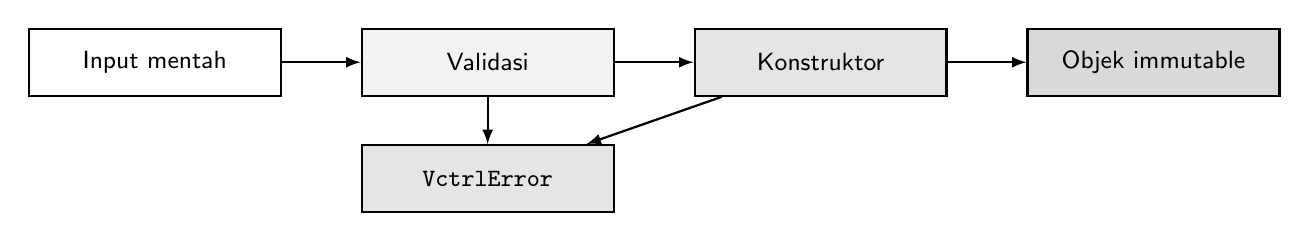
\begin{tikzpicture}[
			node distance=0.6cm and 1.0cm,
			box/.style={rectangle, draw=black, thick, minimum width=3.2cm, minimum height=0.85cm, align=center, font=\sffamily\small},
			err/.style={rectangle, draw=black, thick, fill=black!10, minimum width=3.2cm, minimum height=0.85cm, align=center, font=\sffamily\small},
			line/.style={draw, thick, -latex}
		]
		\node[box, fill=white] (input) {Input mentah};
		\node[box, fill=black!5, right=of input] (valid) {Validasi};
		\node[box, fill=black!10, right=of valid] (ctor) {Konstruktor};
		\node[box, fill=black!15, right=of ctor] (obj) {Objek immutable};
		\node[err, below=of valid] (err1) {\texttt{VctrlError}};

		\draw[line] (input) -- (valid);
		\draw[line] (valid) -- (ctor);
		\draw[line] (ctor) -- (obj);
		\draw[line] (valid) -- (err1);
		\draw[line] (ctor) -- (err1);
	\end{tikzpicture}
	\caption{Alur validasi dan konstruksi objek kontrak.}
	\label{fig:validasi}
\end{figure}

\section{Format Biner Byte-Level}

\subsection{Spesifikasi Format}

\texttt{BinaryEncoder} menulis byte stream dengan layout deterministik. Semua integer little-endian. Panjang string diawali \texttt{u8}. Version byte saat ini bernilai \texttt{3}. Tabel~\ref{tab:format} mencantumkan layout per tipe.

\begin{table}[H]
	\centering
	\caption{Layout byte-level format biner versi 3.}
	\label{tab:format}
	\footnotesize
	\begin{tabularx}{\textwidth}{l X}
		\toprule
		Tipe & Layout \\
		\midrule
		\texttt{Blob} & \texttt{u8 version | u64 LE data\_len | data[data\_len]} \\
		\texttt{Tree} & \texttt{u8 version | u32 LE count | entry[count]} \\
		\texttt{entry} & \texttt{u8 name\_len | name[name\_len] | u8 kind | u8 hash[64]} \\
		\texttt{Commit} & \texttt{u8 version | u8 tree[64] | u16 LE parent\_count} \\
		 & \texttt{| parent[parent\_count][64] | u8 author\_name\_len} \\
		 & \texttt{| author\_name | u8 author\_email\_len | author\_email} \\
		 & \texttt{| u8 committer\_name\_len | committer\_name} \\
		 & \texttt{| u8 committer\_email\_len | committer\_email} \\
		 & \texttt{| u32 LE msg\_len | msg | i64 LE timestamp} \\
		 & \texttt{| i16 LE tz\_offset | u8 enc\_len | enc} \\
		\texttt{Tag} & \texttt{u8 version | u8 name\_len | name} \\
		 & \texttt{| u8 target[64] | u8 has\_tagger | [tagger]} \\
		 & \texttt{| u32 LE msg\_len | msg | i64 LE timestamp} \\
		 & \texttt{| i16 LE tz\_offset | u8 enc\_len | enc} \\
		\bottomrule
	\end{tabularx}
\end{table}

Nilai \texttt{kind} pada entri tree: \texttt{0} untuk \texttt{Blob}, \texttt{1} untuk \texttt{Executable}, \texttt{2} untuk \texttt{Symlink}, \texttt{3} untuk \texttt{Tree}, \texttt{4} untuk \texttt{Submodule}. Nilai \texttt{has\_tagger} pada tag: \texttt{0} untuk absen, \texttt{1} untuk hadir.

Gambar~\ref{fig:binformat} menunjukkan layout blob dan tree secara visual.

\begin{figure}[H]
	\centering
	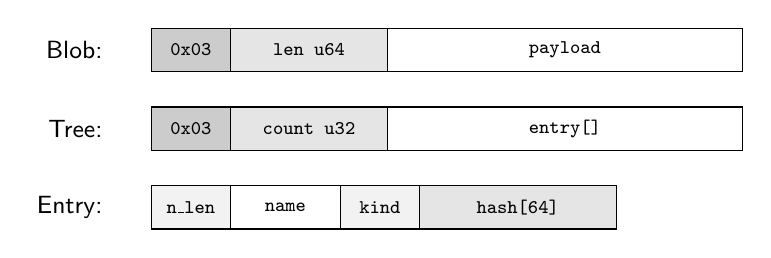
\begin{tikzpicture}[
			cell/.style={rectangle, draw=black, minimum height=0.55cm, font=\ttfamily\scriptsize, align=center},
			lbl/.style={font=\sffamily\small, anchor=east}
		]
		\node[lbl] at (-0.3, 1.4) {Blob:};
		\node[cell, fill=black!20, minimum width=1.0cm] (b1) at (0.7, 1.4) {0x03};
		\node[cell, fill=black!10, minimum width=2.0cm] (b2) at (2.2, 1.4) {len u64};
		\node[cell, fill=white, minimum width=4.5cm] (b3) at (5.45, 1.4) {payload};

		\node[lbl] at (-0.3, 0.4) {Tree:};
		\node[cell, fill=black!20, minimum width=1.0cm] (t1) at (0.7, 0.4) {0x03};
		\node[cell, fill=black!10, minimum width=2.0cm] (t2) at (2.2, 0.4) {count u32};
		\node[cell, fill=white, minimum width=4.5cm] (t3) at (5.45, 0.4) {entry[]};

		\node[lbl] at (-0.3, -0.6) {Entry:};
		\node[cell, fill=black!5, minimum width=1.0cm] (e1) at (0.7, -0.6) {n\_len};
		\node[cell, fill=white, minimum width=1.4cm] (e2) at (1.9, -0.6) {name};
		\node[cell, fill=black!5, minimum width=1.0cm] (e3) at (3.1, -0.6) {kind};
		\node[cell, fill=black!10, minimum width=2.5cm] (e4) at (4.85, -0.6) {hash[64]};
	\end{tikzpicture}
	\caption{Layout byte-level untuk \texttt{Blob}, \texttt{Tree}, dan \texttt{TreeEntry}.}
	\label{fig:binformat}
\end{figure}

\subsection{Batasan Decoder}

\texttt{BinaryDecoder} menerapkan pertahanan berlapis. Input dibaca dengan \texttt{read\_bounded} yang memakai buffer 4 KiB dan menolak alokasi melebihi batas per tipe. Setiap offset diperiksa sebelum slicing. Setiap string divalidasi UTF-8. Setiap nilai numerik dikonversi dengan \texttt{try\_from} sehingga overflow terdeteksi sebelum alokasi. Batas \texttt{MAX\_*} diperiksa ulang setelah konversi.

Decoder menolak: version byte yang bukan \texttt{3}, panjang yang tidak cocok, trailing bytes setelah payload, kind byte yang tidak dikenal, dan tagger presence byte yang bukan \texttt{0} atau \texttt{1}.

\section{Implementasi Referensi: libvctrl\_core}

\subsection{BinaryEncoder dan BinaryDecoder}

Keduanya tipe zero-sized. \texttt{BinaryEncoder} mengimplementasikan \texttt{Encoder}. \texttt{BinaryDecoder} mengimplementasikan \texttt{Decoder}. Pemakaian ditunjukkan pada blok kode berikut.

\begin{lstlisting}[style=code]
use std::io::Cursor;
use libvctrl_core::codec::{BinaryDecoder, BinaryEncoder};
use libvctrl_handler::{Blob, Decoder, Encoder, VctrlError};

fn roundtrip() -> Result<(), VctrlError> {
    let blob = Blob::new(b"halo".to_vec())?;
    let mut buf = Vec::new();
    BinaryEncoder.encode_blob(&blob, &mut buf)?;
    let out = BinaryDecoder.decode_blob(Cursor::new(buf))?;
    assert_eq!(out.data(), blob.data());
    Ok(())
}
\end{lstlisting}

\subsection{Sha512Hasher}

\texttt{Sha512Hasher} adalah adapter zero-sized dari \texttt{libvctrl\_sha512::Hash} ke \texttt{Hasher}. Tipe ini membaca input dalam chunk 4 KiB dan mengembalikan \texttt{Hash} 64 byte. Pemakaian ditunjukkan pada blok kode berikut.

\begin{lstlisting}[style=code]
use libvctrl_core::hash::Sha512Hasher;
use libvctrl_handler::{Hasher, VctrlError};

fn hash() -> Result<(), VctrlError> {
    let hasher = Sha512Hasher;
    let digest = hasher.hash(b"konten".as_ref())?;
    assert_eq!(digest.as_bytes().len(), 64);
    Ok(())
}
\end{lstlisting}

\subsection{Builder}

Lima builder tersedia. Tabel~\ref{tab:builder} mencantumkan tanda tangan metode.

\begin{table}[H]
	\centering
	\caption{Metode builder pada \texttt{libvctrl\_core::object}.}
	\label{tab:builder}
	\footnotesize
	\begin{tabularx}{\textwidth}{l X}
		\toprule
		Builder & Metode \\
		\midrule
		\texttt{BlobBuilder} & \texttt{new()}, \texttt{with\_data(Vec<u8>)}, \texttt{build() -> Result<Blob, \_>} \\
		\texttt{TreeEntryBuilder} & \texttt{new(String, EntryKind, Hash)}, \texttt{build() -> Result<TreeEntry, \_>} \\
		\texttt{TreeBuilder} & \texttt{new()}, \texttt{entry(TreeEntry)}, \texttt{add\_entry(String, EntryKind, Hash)}, \texttt{build()} \\
		\texttt{CommitBuilder} & \texttt{new()}, \texttt{tree(Hash)}, \texttt{parent(Hash)}, \texttt{author(UserID)}, \texttt{committer(UserID)}, \texttt{message(impl Into<String>)}, \texttt{meta(CommitMeta)}, \texttt{build()} \\
		\texttt{TagBuilder} & \texttt{new()}, \texttt{name(impl Into<String>)}, \texttt{target(Hash)}, \texttt{tagger(UserID)}, \texttt{message(impl Into<String>)}, \texttt{meta(CommitMeta)}, \texttt{build()} \\
		\bottomrule
	\end{tabularx}
\end{table}

Builder memvalidasi field wajib pada \texttt{build()}. Jika field wajib absen, \texttt{build()} mengembalikan \texttt{VctrlError::Other}. Contoh ditunjukkan pada blok kode berikut.

\begin{lstlisting}[style=code]
use libvctrl_core::object::{CommitBuilder, TreeBuilder, TreeEntryBuilder};
use libvctrl_handler::{EntryKind, Hash, UserID, VctrlError};

fn build() -> Result<(), VctrlError> {
    let hash = Hash::from_bytes(&[1u8; 64])?;
    let entry = TreeEntryBuilder::new(
        "a.txt".to_string(), EntryKind::Blob, hash,
    ).build()?;
    let tree = TreeBuilder::new().entry(entry).build()?;
    let user = UserID::new(
        "Alice".to_string(), "alice@example.com".to_string(),
    )?;
    let commit = CommitBuilder::new()
        .tree(hash)
        .author(user.clone())
        .committer(user)
        .message("pesan")
        .build()?;
    assert_eq!(commit.message(), "pesan");
    let _ = tree;
    Ok(())
}
\end{lstlisting}

\subsection{In-Memory Store}

\texttt{MemoryStore} mengimplementasikan \texttt{ObjectStore} dengan \texttt{HashMap<Hash, Vec<u8>>}. \texttt{MemoryRefStore} mengimplementasikan \texttt{RefStore} dengan \texttt{HashMap<String, Hash>}. Keduanya cocok untuk pengujian dan prototipe. Contoh ditunjukkan pada blok kode berikut.

\begin{lstlisting}[style=code]
use std::io::Read;
use libvctrl_core::store::{MemoryRefStore, MemoryStore};
use libvctrl_handler::{Hash, ObjectStore, RefStore, VctrlError};

fn store() -> Result<(), VctrlError> {
    let mut objects = MemoryStore::new();
    let mut refs = MemoryRefStore::new();
    let hash = Hash::from_bytes(&[2u8; 64])?;
    objects.put(&hash, b"data")?;
    refs.set_ref("refs/heads/main", &hash)?;
    let mut buf = Vec::new();
    objects.get(&hash)?.read_to_end(&mut buf)?;
    assert_eq!(buf, b"data");
    Ok(())
}
\end{lstlisting}

Gambar~\ref{fig:encodehash} menunjukkan siklus encode, hash, simpan, dan bangun ulang.

\begin{figure}[H]
	\centering
	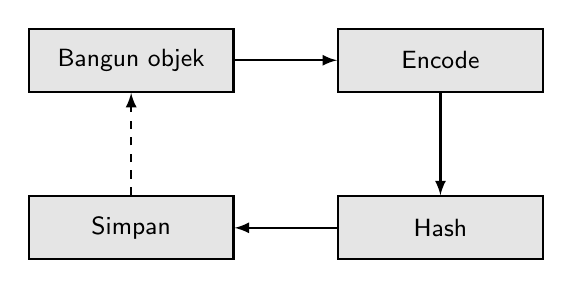
\begin{tikzpicture}[
			node distance=1.3cm,
			box/.style={rectangle, draw=black, thick, fill=black!10, minimum width=2.6cm, minimum height=0.8cm, align=center, font=\sffamily\small},
			line/.style={draw, thick, -latex}
		]
		\node[box] (build) {Bangun objek};
		\node[box, right=of build] (encode) {Encode};
		\node[box, below=of encode] (hash) {Hash};
		\node[box, left=of hash] (store) {Simpan};

		\draw[line] (build) -- (encode);
		\draw[line] (encode) -- (hash);
		\draw[line] (hash) -- (store);
		\draw[line, dashed] (store) -- (build);
	\end{tikzpicture}
	\caption{Siklus encode, hash, simpan, dan bangun ulang objek.}
	\label{fig:encodehash}
\end{figure}

\section{Kriptografi: libvctrl\_sha512}

\subsection{Primitif dan Feature Flags}

\texttt{libvctrl\_sha512} menyediakan SHA-512, HMAC-SHA512, dan HKDF-SHA512. Modul \texttt{sha384} tersedia jika fitur \texttt{sha384} aktif (default). Fitur \texttt{opt\_size} mengubah strategi inlining round function untuk mengurangi ukuran binary. Crate ini \texttt{no\_std} ketika dibangun di luar target test. Satu-satunya dependensi eksternal adalah \texttt{zeroize} dengan \texttt{default-features = false}.

Tabel~\ref{tab:kripto} mencantumkan tanda tangan metode utama.

\begin{table}[H]
	\centering
	\caption{Tanda tangan API kriptografi.}
	\label{tab:kripto}
	\footnotesize
	\begin{tabularx}{\textwidth}{l X l}
		\toprule
		Tipe & Metode & Keluaran \\
		\midrule
		\texttt{Hash} & \texttt{new()}, \texttt{update(impl AsRef<[u8]>)}, \texttt{finalize()}, \texttt{hash(impl AsRef<[u8]>)} & \texttt{[u8; 64]} \\
		\texttt{Hash} & \texttt{verify(self, \&[u8; 64]) -> bool} & \texttt{bool} \\
		\texttt{HMAC} & \texttt{mac(T, U) -> [u8; 64]}, \texttt{new(impl AsRef<[u8]>)} & \texttt{[u8; 64]} \\
		\texttt{HMAC} & \texttt{finalize\_verify(self, \&[u8; 64]) -> bool} & \texttt{bool} \\
		\texttt{HKDF} & \texttt{extract(salt, ikm) -> [u8; 64]} & \texttt{[u8; 64]} \\
		\texttt{HKDF} & \texttt{expand(\&mut [u8], prk, info)} & \texttt{()} \\
		\texttt{sha384::Hash} & \texttt{hash}, \texttt{update}, \texttt{finalize} & \texttt{[u8; 48]} \\
		\bottomrule
	\end{tabularx}
\end{table}

\subsection{Contoh HMAC dan HKDF}

Blok kode berikut menunjukkan autentikasi pesan dan derivasi kunci.

\begin{lstlisting}[style=code]
use libvctrl_sha512::{HKDF, HMAC};

fn kripto() {
    let tag = HMAC::mac(b"pesan", b"kunci");
    assert!(HMAC::verify(b"pesan", b"kunci", &tag));

    let prk = HKDF::extract(b"salt", b"input");
    let mut out = [0u8; 32];
    HKDF::expand(&mut out, prk, b"konteks");
    assert_eq!(out.len(), 32);
}
\end{lstlisting}

\section{Fasad dan Plumbing}

\subsection{Re-export Fasad}

\texttt{libvctrl} mengekspor ulang \texttt{handler}, \texttt{reference}, dan \texttt{crypto} sebagai namespace. Namespace \texttt{crypto} memisahkan \texttt{libvctrl\_sha512::Hash} (hasher) dari \texttt{libvctrl\_handler::Hash} (content address). Pemakai yang mengimpor keduanya harus memakai alias.

\subsection{Repository}

\texttt{Repository} menyediakan API tingkat tinggi untuk commit, snapshot, baca objek, dan kelola cabang. Tabel~\ref{tab:repository} mencantumkan tanda tangan metode.

\begin{table}[H]
	\centering
	\caption{Tanda tangan metode \texttt{Repository}.}
	\label{tab:repository}
	\footnotesize
	\begin{tabularx}{\textwidth}{l X}
		\toprule
		Metode & Tanda tangan \\
		\midrule
		\texttt{new} & \texttt{new(Box<dyn ObjectStore>, Box<dyn RefStore>) -> Self} \\
		\texttt{commit} & \texttt{commit(\&mut self, \&str, impl IntoIterator<Item=FileToCommit>, impl Into<String>, UserID) -> Result<Hash, \_>} \\
		\texttt{snapshot} & \texttt{snapshot(\&mut self, impl IntoIterator<Item=FileToCommit>) -> Result<Hash, \_>} \\
		\texttt{read\_blob} & \texttt{read\_blob(\&self, \&Hash) -> Result<Blob, \_>} \\
		\texttt{read\_tree} & \texttt{read\_tree(\&self, \&Hash) -> Result<Tree, \_>} \\
		\texttt{read\_commit} & \texttt{read\_commit(\&self, \&Hash) -> Result<Commit, \_>} \\
		\texttt{head} & \texttt{head(\&self, \&str) -> Result<Hash, \_>} \\
		\texttt{branches} & \texttt{branches(\&self) -> Result<Vec<String>, \_>} \\
		\texttt{log} & \texttt{log(\&self, \&str) -> Result<Vec<(Hash, Commit)>, \_>} \\
		\texttt{file\_at} & \texttt{file\_at(\&self, \&Hash, \&str) -> Result<Option<Vec<u8>>, \_>} \\
		\texttt{create\_branch} & \texttt{create\_branch(\&mut self, \&str, \&Hash) -> Result<(), \_>} \\
		\texttt{delete\_branch} & \texttt{delete\_branch(\&mut self, \&str) -> Result<(), \_>} \\
		\bottomrule
	\end{tabularx}
\end{table}

\texttt{FileToCommit} menyediakan tiga konstruktor: \texttt{blob(path, data)}, \texttt{executable(path, data)}, dan \texttt{symlink(path, target)}. Tipe ini memuat \texttt{path: String}, \texttt{kind: EntryKind}, dan \texttt{data: Vec<u8>}.

\subsection{cat\_file dan cat\_file\_batch}

\texttt{libvctrl\_plumbing} menyediakan dua fungsi tingkat perintah. Tabel~\ref{tab:catfile} mencantumkan mode dan keluaran.

\begin{table}[H]
	\centering
	\caption{Mode \texttt{CatFileMode} dan keluarannya.}
	\label{tab:catfile}
	\footnotesize
	\begin{tabularx}{\textwidth}{l X}
		\toprule
		Mode & Keluaran \\
		\midrule
		\texttt{Exists} & Tidak ada output, sukses jika objek ada \\
		\texttt{ObjectType} & Nama tipe diikuti newline \\
		\texttt{ObjectSize} & Ukuran payload dalam byte \\
		\texttt{PrettyPrint} & Representasi teks objek \\
		\texttt{Raw(ObjectType)} & Byte payload mentah, gagal jika tipe tidak cocok \\
		\bottomrule
	\end{tabularx}
\end{table}

\texttt{BatchOptions} memuat field \texttt{format: Option<String>}, \texttt{nul\_terminated: bool}, \texttt{follow\_symlinks: bool}, \texttt{buffer: bool}, dan \texttt{print\_contents: bool}. Format string mendukung placeholder \texttt{\%(objectname)}, \texttt{\%(objecttype)}, dan \texttt{\%(objectsize)}.

Contoh pemakaian ditunjukkan pada blok kode berikut.

\begin{lstlisting}[style=code]
use libvctrl_plumbing::cat_file::{cat_file, CatFileMode};
use libvctrl::{BinaryDecoder, Hash, MemoryStore, VctrlError};

fn cat(store: &MemoryStore, hash: &Hash)
    -> Result<(), VctrlError>
{
    let decoder = BinaryDecoder;
    let mut out = Vec::new();
    cat_file(
        store, &decoder, &hash.to_string(),
        CatFileMode::PrettyPrint, &mut out,
    )?;
    assert!(!out.is_empty());
    Ok(())
}
\end{lstlisting}

Keluaran \texttt{PrettyPrint} untuk objek blob mengikuti format berikut.

\begin{lstlisting}[style=out]
halo
\end{lstlisting}

\section{Template Implementasi Backend Kustom}

\subsection{Kontrak yang Harus Dipenuhi}

Backend kustom yang ingin dipakai bersama \texttt{Repository} harus mengimplementasikan \texttt{ObjectStore} dan \texttt{RefStore}. Keduanya memiliki bound \texttt{Send + Sync}. Backend boleh mengimplementasikan trait lain seperti \texttt{Index} atau \texttt{RevWalk} jika diperlukan. Tabel~\ref{tab:backend} mencantumkan checklist implementasi.

\begin{table}[H]
	\centering
	\caption{Checklist implementasi backend kustom.}
	\label{tab:backend}
	\footnotesize
	\begin{tabularx}{\textwidth}{l X}
		\toprule
		Item & Kewajiban \\
		\midrule
		\texttt{put} & Menyimpan byte mentah dengan kunci \texttt{Hash}, idempoten \\
		\texttt{get} & Mengembalikan \texttt{Box<dyn Read + Send + '\_>} yang membaca byte \\
		\texttt{delete} & Menghapus entri jika ada, idempoten \\
		\texttt{exists} & Mengembalikan \texttt{false} tanpa error jika tidak ada \\
		\texttt{set\_ref} & Memvalidasi nama via \texttt{validate\_ref\_name} \\
		\texttt{get\_ref} & Mengembalikan \texttt{RefNotFound} jika nama tidak ada \\
		\texttt{delete\_ref} & Menghapus ref jika ada, idempoten \\
		\texttt{list\_refs} & Mengembalikan vektor nama yang terurut \\
		Bound & \texttt{impl ObjectStore for MyStore} dengan \texttt{MyStore: Send + Sync} \\
		\bottomrule
	\end{tabularx}
\end{table}

\subsection{Template Implementasi}

Template berikut menunjukkan pola implementasi dengan \texttt{Mutex} internal. Pola ini dipakai \texttt{MonumentumStore}.

\begin{lstlisting}[style=code]
use std::io::{Cursor, Read};
use std::sync::Mutex;
use libvctrl_handler::{
    Hash, ObjectStore, RefStore, VctrlError, validate_ref_name,
};

pub struct MyStore {
    objects: Mutex<std::collections::HashMap<Hash, Vec<u8>>>,
    refs: Mutex<std::collections::HashMap<String, Hash>>,
}

impl ObjectStore for MyStore {
    fn put(&mut self, hash: &Hash, data: &[u8])
        -> Result<(), VctrlError>
    {
        self.objects.lock()
            .map_err(|_| VctrlError::Other("lock".into()))?
            .insert(*hash, data.to_vec());
        Ok(())
    }

    fn get(&self, hash: &Hash)
        -> Result<Box<dyn Read + Send + '_>, VctrlError>
    {
        let guard = self.objects.lock()
            .map_err(|_| VctrlError::Other("lock".into()))?;
        let bytes = guard.get(hash)
            .ok_or(VctrlError::ObjectNotFound(*hash))?
            .clone();
        Ok(Box::new(Cursor::new(bytes)))
    }

    fn delete(&mut self, hash: &Hash) -> Result<(), VctrlError> {
        self.objects.lock()
            .map_err(|_| VctrlError::Other("lock".into()))?
            .remove(hash);
        Ok(())
    }

    fn exists(&self, hash: &Hash) -> Result<bool, VctrlError> {
        Ok(self.objects.lock()
            .map_err(|_| VctrlError::Other("lock".into()))?
            .contains_key(hash))
    }
}

impl RefStore for MyStore {
    fn set_ref(&mut self, name: &str, hash: &Hash)
        -> Result<(), VctrlError>
    {
        validate_ref_name(name)?;
        self.refs.lock()
            .map_err(|_| VctrlError::Other("lock".into()))?
            .insert(name.to_string(), *hash);
        Ok(())
    }

    fn get_ref(&self, name: &str) -> Result<Hash, VctrlError> {
        self.refs.lock()
            .map_err(|_| VctrlError::Other("lock".into()))?
            .get(name).copied()
            .ok_or_else(|| VctrlError::RefNotFound(name.into()))
    }

    fn delete_ref(&mut self, name: &str)
        -> Result<(), VctrlError>
    {
        self.refs.lock()
            .map_err(|_| VctrlError::Other("lock".into()))?
            .remove(name);
        Ok(())
    }

    fn list_refs(&self) -> Result<Vec<String>, VctrlError> {
        let mut names: Vec<String> = self.refs.lock()
            .map_err(|_| VctrlError::Other("lock".into()))?
            .keys().cloned().collect();
        names.sort();
        Ok(names)
    }
}
\end{lstlisting}

Gambar~\ref{fig:backend} menunjukkan posisi backend sebagai implementasi trait.

\begin{figure}[H]
	\centering
	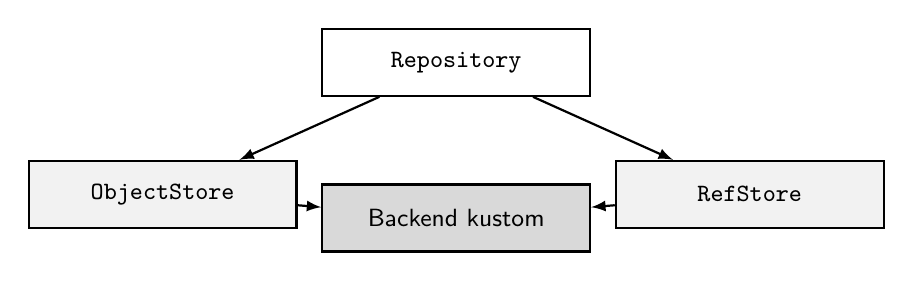
\begin{tikzpicture}[
			box/.style={rectangle, draw=black, thick, minimum width=3.4cm, minimum height=0.85cm, align=center, font=\sffamily\small},
			line/.style={draw, thick, -latex}
		]
		\node[box, fill=white] (repo) {\texttt{Repository}};
		\node[box, fill=black!5, below left=0.8cm and 0.3cm of repo] (obj) {\texttt{ObjectStore}};
		\node[box, fill=black!5, below right=0.8cm and 0.3cm of repo] (ref) {\texttt{RefStore}};
		\node[box, fill=black!15, below=1.1cm of repo] (mon) {Backend kustom};

		\draw[line] (repo) -- (obj);
		\draw[line] (repo) -- (ref);
		\draw[line] (obj) -- (mon);
		\draw[line] (ref) -- (mon);
	\end{tikzpicture}
	\caption{Integrasi backend kustom melalui trait penyimpanan.}
	\label{fig:backend}
\end{figure}

\section{Studi Kasus: Commit End-to-End}

\subsection{Langkah 1: Siapkan Store}

Gunakan \texttt{MemoryStore} dan \texttt{MemoryRefStore} sebagai backend minimal.

\begin{lstlisting}[style=code]
use libvctrl::{MemoryRefStore, MemoryStore, Repository};

let mut repo = Repository::new(
    Box::new(MemoryStore::new()),
    Box::new(MemoryRefStore::new()),
);
\end{lstlisting}

\subsection{Langkah 2: Buat UserID}

Buat identitas penulis. Email wajib memuat \texttt{@}.

\begin{lstlisting}[style=code]
use libvctrl::UserID;

let user = UserID::new(
    "Alice".to_string(), "alice@example.com".to_string(),
)?;
\end{lstlisting}

\subsection{Langkah 3: Siapkan Berkas}

Bungkus isi berkas menjadi \texttt{FileToCommit}.

\begin{lstlisting}[style=code]
use libvctrl::FileToCommit;

let files = vec![
    FileToCommit::blob("catatan.md", b"halo".to_vec()),
];
\end{lstlisting}

\subsection{Langkah 4: Commit}

Panggil \texttt{commit} pada cabang utama.

\begin{lstlisting}[style=code]
let commit = repo.commit(
    "refs/heads/main", files, "commit pertama", user,
)?;
\end{lstlisting}

\subsection{Langkah 5: Baca HEAD}

Periksa hash ujung cabang.

\begin{lstlisting}[style=code]
let head = repo.head("refs/heads/main")?;
assert_eq!(head, commit);
\end{lstlisting}

\subsection{Langkah 6: Baca Berkas pada Commit}

Baca isi berkas pada commit tertentu.

\begin{lstlisting}[style=code]
let isi = repo.file_at(&commit, "catatan.md")?;
assert!(isi.is_some());
\end{lstlisting}

\subsection{Langkah 7: Lihat Log}

Telusuri riwayat commit.

\begin{lstlisting}[style=code]
let log = repo.log("refs/heads/main")?;
assert_eq!(log.len(), 1);
\end{lstlisting}

\subsection{Langkah 8: Buat Cabang}

Buat cabang baru dari commit yang sudah ada.

\begin{lstlisting}[style=code]
repo.create_branch("refs/heads/dev", &commit)?;
assert_eq!(repo.head("refs/heads/dev")?, commit);
\end{lstlisting}

\subsection{Langkah 9: Snapshot Tanpa Commit}

Buat tree tanpa membuat commit, berguna untuk preview.

\begin{lstlisting}[style=code]
let tree_hash = repo.snapshot(vec![
    FileToCommit::blob("catatan.md", b"halo".to_vec()),
])?;
assert_eq!(tree_hash.as_bytes().len(), 64);
\end{lstlisting}

\subsection{Langkah 10: Commit Kedua}

Commit kedua memakai HEAD cabang sebagai parent otomatis.

\begin{lstlisting}[style=code]
let commit2 = repo.commit(
    "refs/heads/main",
    vec![FileToCommit::blob("catatan.md", b"halo 2".to_vec())],
    "commit kedua",
    UserID::new(
        "Alice".to_string(), "alice@example.com".to_string(),
    )?,
)?;
let log = repo.log("refs/heads/main")?;
assert_eq!(log.len(), 2);
assert_eq!(log.first().map(|(h, _)| *h), Some(commit2));
\end{lstlisting}

Gambar~\ref{fig:commit} menunjukkan lima langkah utama di dalam \texttt{Repository::commit}.

\begin{figure}[H]
	\centering
	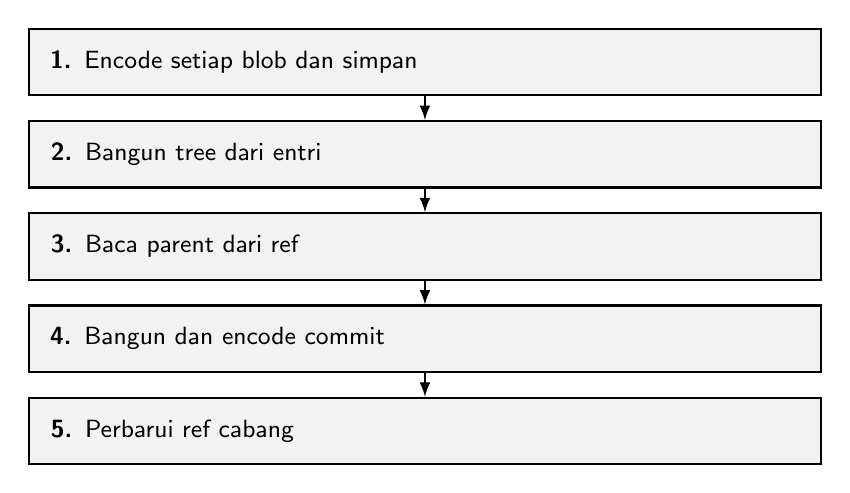
\begin{tikzpicture}[
			pstep/.style={rectangle, draw=black, thick, fill=black!5, text width=9.5cm, align=left, minimum height=0.7cm, font=\sffamily\small, inner sep=8pt},
			line/.style={draw, thick, -latex}
		]
		\node[pstep] (s1) {\textbf{1.} Encode setiap blob dan simpan};
		\node[pstep, below=0.3cm of s1] (s2) {\textbf{2.} Bangun tree dari entri};
		\node[pstep, below=0.3cm of s2] (s3) {\textbf{3.} Baca parent dari ref};
		\node[pstep, below=0.3cm of s3] (s4) {\textbf{4.} Bangun dan encode commit};
		\node[pstep, below=0.3cm of s4] (s5) {\textbf{5.} Perbarui ref cabang};

		\draw[line] (s1) -- (s2);
		\draw[line] (s2) -- (s3);
		\draw[line] (s3) -- (s4);
		\draw[line] (s4) -- (s5);
	\end{tikzpicture}
	\caption{Lima langkah utama \texttt{Repository::commit}.}
	\label{fig:commit}
\end{figure}

\section{Kesalahan Umum dan Cara Menghindarinya}

Tabel~\ref{tab:kesalahan} merangkum pemicu error dan perbaikannya.

\begin{table}[H]
	\centering
	\caption{Pemicu error umum dan perbaikannya.}
	\label{tab:kesalahan}
	\footnotesize
	\begin{tabularx}{\textwidth}{X l X}
		\toprule
		Pemicu & Varian & Perbaikan \\
		\midrule
		Hash kurang dari 64 byte & \texttt{InvalidHashLength} & Pakai array \texttt{[u8; 64]} \\
		Nama entri memuat \texttt{/} & \texttt{InvalidName} & Pecah jadi tree bertingkat \\
		Ref diawali \texttt{.} atau \texttt{/} & \texttt{InvalidName} & Pakai \texttt{refs/heads/...} \\
		Parent duplikat & \texttt{DuplicateParent} & Deduplikasi sebelum \texttt{Commit::new} \\
		Pesan melebihi 1 MiB & \texttt{ExceededMaxSize} & Perpendek pesan \\
		Offset zona waktu $>$ 1440 & \texttt{InvalidTimezoneOffset} & Pakai menit, rentang $\pm 1440$ \\
		Email tanpa \texttt{@} & \texttt{InvalidEmail} & Validasi sebelum \texttt{UserID::new} \\
		\texttt{get} sebelum \texttt{put} & \texttt{ObjectNotFound} & Simpan objek terlebih dahulu \\
		Version byte bukan 3 & \texttt{CorruptedData} & Re-encode dengan encoder versi 3 \\
		Trailing byte setelah payload & \texttt{CorruptedData} & Pastikan panjang prefix akurat \\
		Kind byte $> 4$ & \texttt{CorruptedData} & Pakai \texttt{EntryKind} yang valid \\
		Tagger presence byte bukan 0/1 & \texttt{CorruptedData} & Normalisasi ke \texttt{0} atau \texttt{1} \\
		\bottomrule
	\end{tabularx}
\end{table}

Kesalahan paling sering pada integrasi baru adalah panjang hash yang salah dan ref name yang tidak lolos \texttt{validate\_ref\_name}. Keduanya bisa dicegah dengan memanggil fungsi validasi sebelum konstruksi dan sebelum \texttt{set\_ref}.

\section{Lembar Rujukan Cepat}

Tabel~\ref{tab:cepat} menjadi lembar rujukan cepat untuk operasi yang paling sering dibutuhkan pengembang.

\begin{table}[H]
	\centering
	\caption{Lembar rujukan cepat API libvctrl.}
	\label{tab:cepat}
	\footnotesize
	\begin{tabularx}{\textwidth}{l X}
		\toprule
		Kebutuhan & API atau tipe \\
		\midrule
		Hash dari byte & \texttt{Hash::from\_bytes(\&[u8])} \\
		Hash ke byte & \texttt{hash.as\_bytes()} \\
		Blob dari \texttt{Vec} & \texttt{Blob::new(Vec<u8>)} \\
		Entri tree & \texttt{TreeEntry::new(String, EntryKind, Hash)} \\
		Tree dari entri & \texttt{Tree::new(Vec<TreeEntry>)} \\
		Commit tanpa meta & \texttt{Commit::new(tree, parents, a, c, msg)} \\
		Commit dengan meta & \texttt{Commit::with\_meta(..., meta)} \\
		Tag anotasi & \texttt{Tag::new(name, target, tagger, msg)} \\
		User valid & \texttt{UserID::new(name, email)} \\
		Encode blob & \texttt{BinaryEncoder.encode\_blob(\&b, \&mut w)} \\
		Decode blob & \texttt{BinaryDecoder.decode\_blob(r)} \\
		Hash stream & \texttt{Sha512Hasher.hash(r)} \\
		Simpan objek & \texttt{ObjectStore::put(\&mut s, \&h, \&d)} \\
		Ambil objek & \texttt{ObjectStore::get(\&s, \&h)} \\
		Simpan ref & \texttt{RefStore::set\_ref(\&mut s, name, \&h)} \\
		Ambil ref & \texttt{RefStore::get\_ref(\&s, name)} \\
		Commit berkas & \texttt{Repository::commit(...)} \\
		Baca berkas & \texttt{Repository::file\_at(\&h, path)} \\
		Log cabang & \texttt{Repository::log(name)} \\
		Tampilkan objek & \texttt{cat\_file(...)} \\
		Mode batch & \texttt{cat\_file\_batch(...)} \\
		Backend Monumentum & \texttt{MonumentumStore::new(engine)} \\
		\bottomrule
	\end{tabularx}
\end{table}

\section{Kesimpulan}

Dokumen ini menyajikan tiga perspektif API libvctrl: kontrak sebagai batas, format biner sebagai spesifikasi, dan backend sebagai titik ekstensi. Tiga prinsip penutup:

\begin{enumerate}
	\item Kontrak adalah batas yang tidak dapat dilanggar. \texttt{libvctrl\_handler} menetapkan tipe, trait, konstanta, dan kondisi error yang harus dipatuhi oleh setiap implementasi. Backend kustom yang melanggar kontrak akan gagal pada \texttt{Repository} atau pada decoder, bukan pada pemanggil.
	\item Format adalah spesifikasi, bukan detail internal. Layout byte-level pada Bagian 4 adalah kontrak publik. Perubahan layout memerlukan versi baru pada version byte dan decoder yang kompatibel.
	\item Ekstensi adalah titik masuk yang terdefinisi. Backend kustom mengimplementasikan \texttt{ObjectStore} dan \texttt{RefStore}, bukan memodifikasi \texttt{libvctrl\_core}. Ekstensi tidak boleh mengubah tipe kontrak atau menambah varian error di luar \texttt{VctrlError}.
\end{enumerate}

Pengembang yang memahami ketiga prinsip ini dapat memakai libvctrl sebagai SDK lengkap, sebagai kumpulan crate terpisah, atau sebagai fondasi untuk backend kustom tanpa risiko melanggar invariant yang dijamin oleh lapisan kontrak.

\newpage
\section*{Referensi}
\addcontentsline{toc}{section}{Referensi}

\begin{thebibliography}{99}

	\bibitem{docsrs}
	libvctrl Contributors. (2026).
	\textit{libvctrl API Documentation}.
	docs.rs.
	\texttt{https://docs.rs/libvctrl}

	\bibitem{handler}
	libvctrl Contributors. (2026).
	\textit{libvctrl\_handler: Contracts for Version Control}.
	docs.rs.
	\texttt{https://docs.rs/libvctrl\_handler}

	\bibitem{core}
	libvctrl Contributors. (2026).
	\textit{libvctrl\_core: Reference Implementations}.
	docs.rs.
	\texttt{https://docs.rs/libvctrl\_core}

	\bibitem{sha}
	libvctrl Contributors. (2026).
	\textit{libvctrl\_sha512: SHA-512, HMAC, HKDF}.
	docs.rs.
	\texttt{https://docs.rs/libvctrl\_sha512}

	\bibitem{plumbing}
	libvctrl Contributors. (2026).
	\textit{libvctrl\_plumbing: Command-Level Operations}.
	docs.rs.
	\texttt{https://docs.rs/libvctrl\_plumbing}

	\bibitem{rustbook}
	Rust Team. (2026).
	\textit{The Rust Programming Language}.
	\texttt{https://doc.rust-lang.org/book/}

	\bibitem{rustapi}
	Rust Team. (2026).
	\textit{Rust API Guidelines}.
	\texttt{https://rust-lang.github.io/api-guidelines/}

	\bibitem{progit}
	Chacon, S., \& Straub, B. (2014).
	\textit{Pro Git} (2nd ed.).
	Apress.
	\texttt{https://git-scm.com/book/}

	\bibitem{fips180}
	National Institute of Standards and Technology. (2015).
	\textit{Secure Hash Standard (SHS)}.
	FIPS PUB 180-4.
	\texttt{https://doi.org/10.6028/NIST.FIPS.180-4}

	\bibitem{rfc2104}
	Krawczyk, H., Bellare, M., \& Canetti, R. (1997).
	\textit{HMAC: Keyed-Hashing for Message Authentication}.
	RFC 2104.
	IETF.
	\texttt{https://www.rfc-editor.org/rfc/rfc2104}

	\bibitem{rfc5869}
	Krawczyk, H., \& Eronen, P. (2010).
	\textit{HKDF: HMAC-based Extract-and-Expand Key Derivation Function}.
	RFC 5869.
	IETF.
	\texttt{https://www.rfc-editor.org/rfc/rfc5869}

\end{thebibliography}

\end{document}